\documentclass[11pt, a4paper]{article}
\usepackage{pdfpages}
\usepackage{parallel}
\usepackage[T2A]{fontenc}
\usepackage{ucs}
\usepackage[utf8x]{inputenc}
\usepackage[polish,english,russian]{babel}
\usepackage{hyperref}
\usepackage{rotating}
\usepackage[inner=2cm,top=1.8cm,outer=2cm,bottom=2.3cm,nohead]{geometry}
\usepackage{listings}
\usepackage{graphicx}
\usepackage{wrapfig}
\usepackage{longtable}
\usepackage{indentfirst}
\usepackage{array}
\usepackage{tikzsymbols}
\usepackage{soul}
\usepackage[ruled,vlined]{algorithm2e}
%\counterwithout{figure}{section} 

\usepackage{url}
\makeatletter
\g@addto@macro{\UrlBreaks}{\UrlOrds}
\makeatother

\newcolumntype{P}[1]{>{\raggedright\arraybackslash}p{#1}}
\frenchspacing
\usepackage{fixltx2e} %text sub- and superscripts
\usepackage{icomma} % коскі ў матэматычным рэжыме
\PreloadUnicodePage{4}

\newcommand{\longpage}{\enlargethispage{\baselineskip}}
\newcommand{\shortpage}{\enlargethispage{-\baselineskip}}

\def\switchlang#1{\expandafter\csname switchlang#1\endcsname}
\def\switchlangbe{
\let\saverefname=\refname%
\def\refname{Літаратура}%
\def\figurename{Іл.}%
}
\def\switchlangen{
\let\saverefname=\refname%
\def\refname{References}%
\def\figurename{Fig.}%
}
\def\switchlangru{
\let\saverefname=\refname%
\let\savefigurename=\figurename%
\def\refname{Литература}%
\def\figurename{Рис.}%
}

\hyphenation{admi-ni-stra-tive}
\hyphenation{ex-pe-ri-ence}
\hyphenation{fle-xi-bi-li-ty}
\hyphenation{Py-thon}
\hyphenation{ma-the-ma-ti-cal}
\hyphenation{re-ported}
\hyphenation{imp-le-menta-tions}
\hyphenation{pro-vides}
\hyphenation{en-gi-neering}
\hyphenation{com-pa-ti-bi-li-ty}
\hyphenation{im-pos-sible}
\hyphenation{desk-top}
\hyphenation{elec-tro-nic}
\hyphenation{com-pa-ny}
\hyphenation{de-ve-lop-ment}
\hyphenation{de-ve-loping}
\hyphenation{de-ve-lop}
\hyphenation{da-ta-ba-se}
\hyphenation{plat-forms}
\hyphenation{or-ga-ni-za-tion}
\hyphenation{pro-gramming}
\hyphenation{in-stru-ments}
\hyphenation{Li-nux}
\hyphenation{sour-ce}
\hyphenation{en-vi-ron-ment}
\hyphenation{Te-le-pathy}
\hyphenation{Li-nux-ov-ka}
\hyphenation{Open-BSD}
\hyphenation{Free-BSD}
\hyphenation{men-ti-on-ed}
\hyphenation{app-li-ca-tion}

\def\progref!#1!{\texttt{#1}}
\renewcommand{\arraystretch}{2} %Іначай формулы ў матрыцы зліпаюцца з лініямі
\usepackage{array}

\def\interview #1 (#2), #3, #4, #5\par{

\section[#1, #3, #4]{#1 -- #3, #4}
\def\qname{LVEE}
\def\aname{#1}
\def\q ##1\par{{\noindent \bf \qname: ##1 }\par}
\def\a{{\noindent \bf \aname: } \def\qname{L}\def\aname{#2}}
}

\def\interview* #1 (#2), #3, #4, #5\par{

\section*{#1\\{\small\rm #3, #4. #5}}
\ifx\ParallelWhichBox\undefined%
    \addcontentsline{toc}{section}{#1, #3, #4}%
\else%
\ifnum\ParallelWhichBox=0%
    \addcontentsline{toc}{section}{#1, #3, #4}%
\fi\fi%

\def\qname{LVEE}
\def\aname{#1}
\def\q ##1\par{{\noindent \bf \qname: ##1 }\par}
\def\a{{\noindent \bf \aname: } \def\qname{L}\def\aname{#2}}
}

\newcommand{\interviewfooter}[1]{
\vskip 1em
\noindent \textit{#1}
}

\switchlang{en}
\begin{document}

\title{1984 "--- Tandy TRS-80 Color Mouse}
\date{}
\author{~}
\maketitle
\selectlanguage{english}

Tandy TRS-80 Color Mouse (fig. \ref{fig:TandyColorMousePic}) was designed for the RadioShack TRS-80 Color Computer (later renamed to Tandy Color Computer). The Color Computer model 1, released in 1981, was a home computer equipped with a calculator rubber keyboard, 4Kb to 32Kb RAM, 8-bit word length, and used a TV set as a display \cite{wiki}. Over time, the list of peripheral devices expanded, and in 1984, a mouse  was added to their list \cite{adv}, designed to be connected to the analog joystick port. The mouse was manufactured under contract by Alps company in Japan.

\begin{figure}[h]
   \centering
    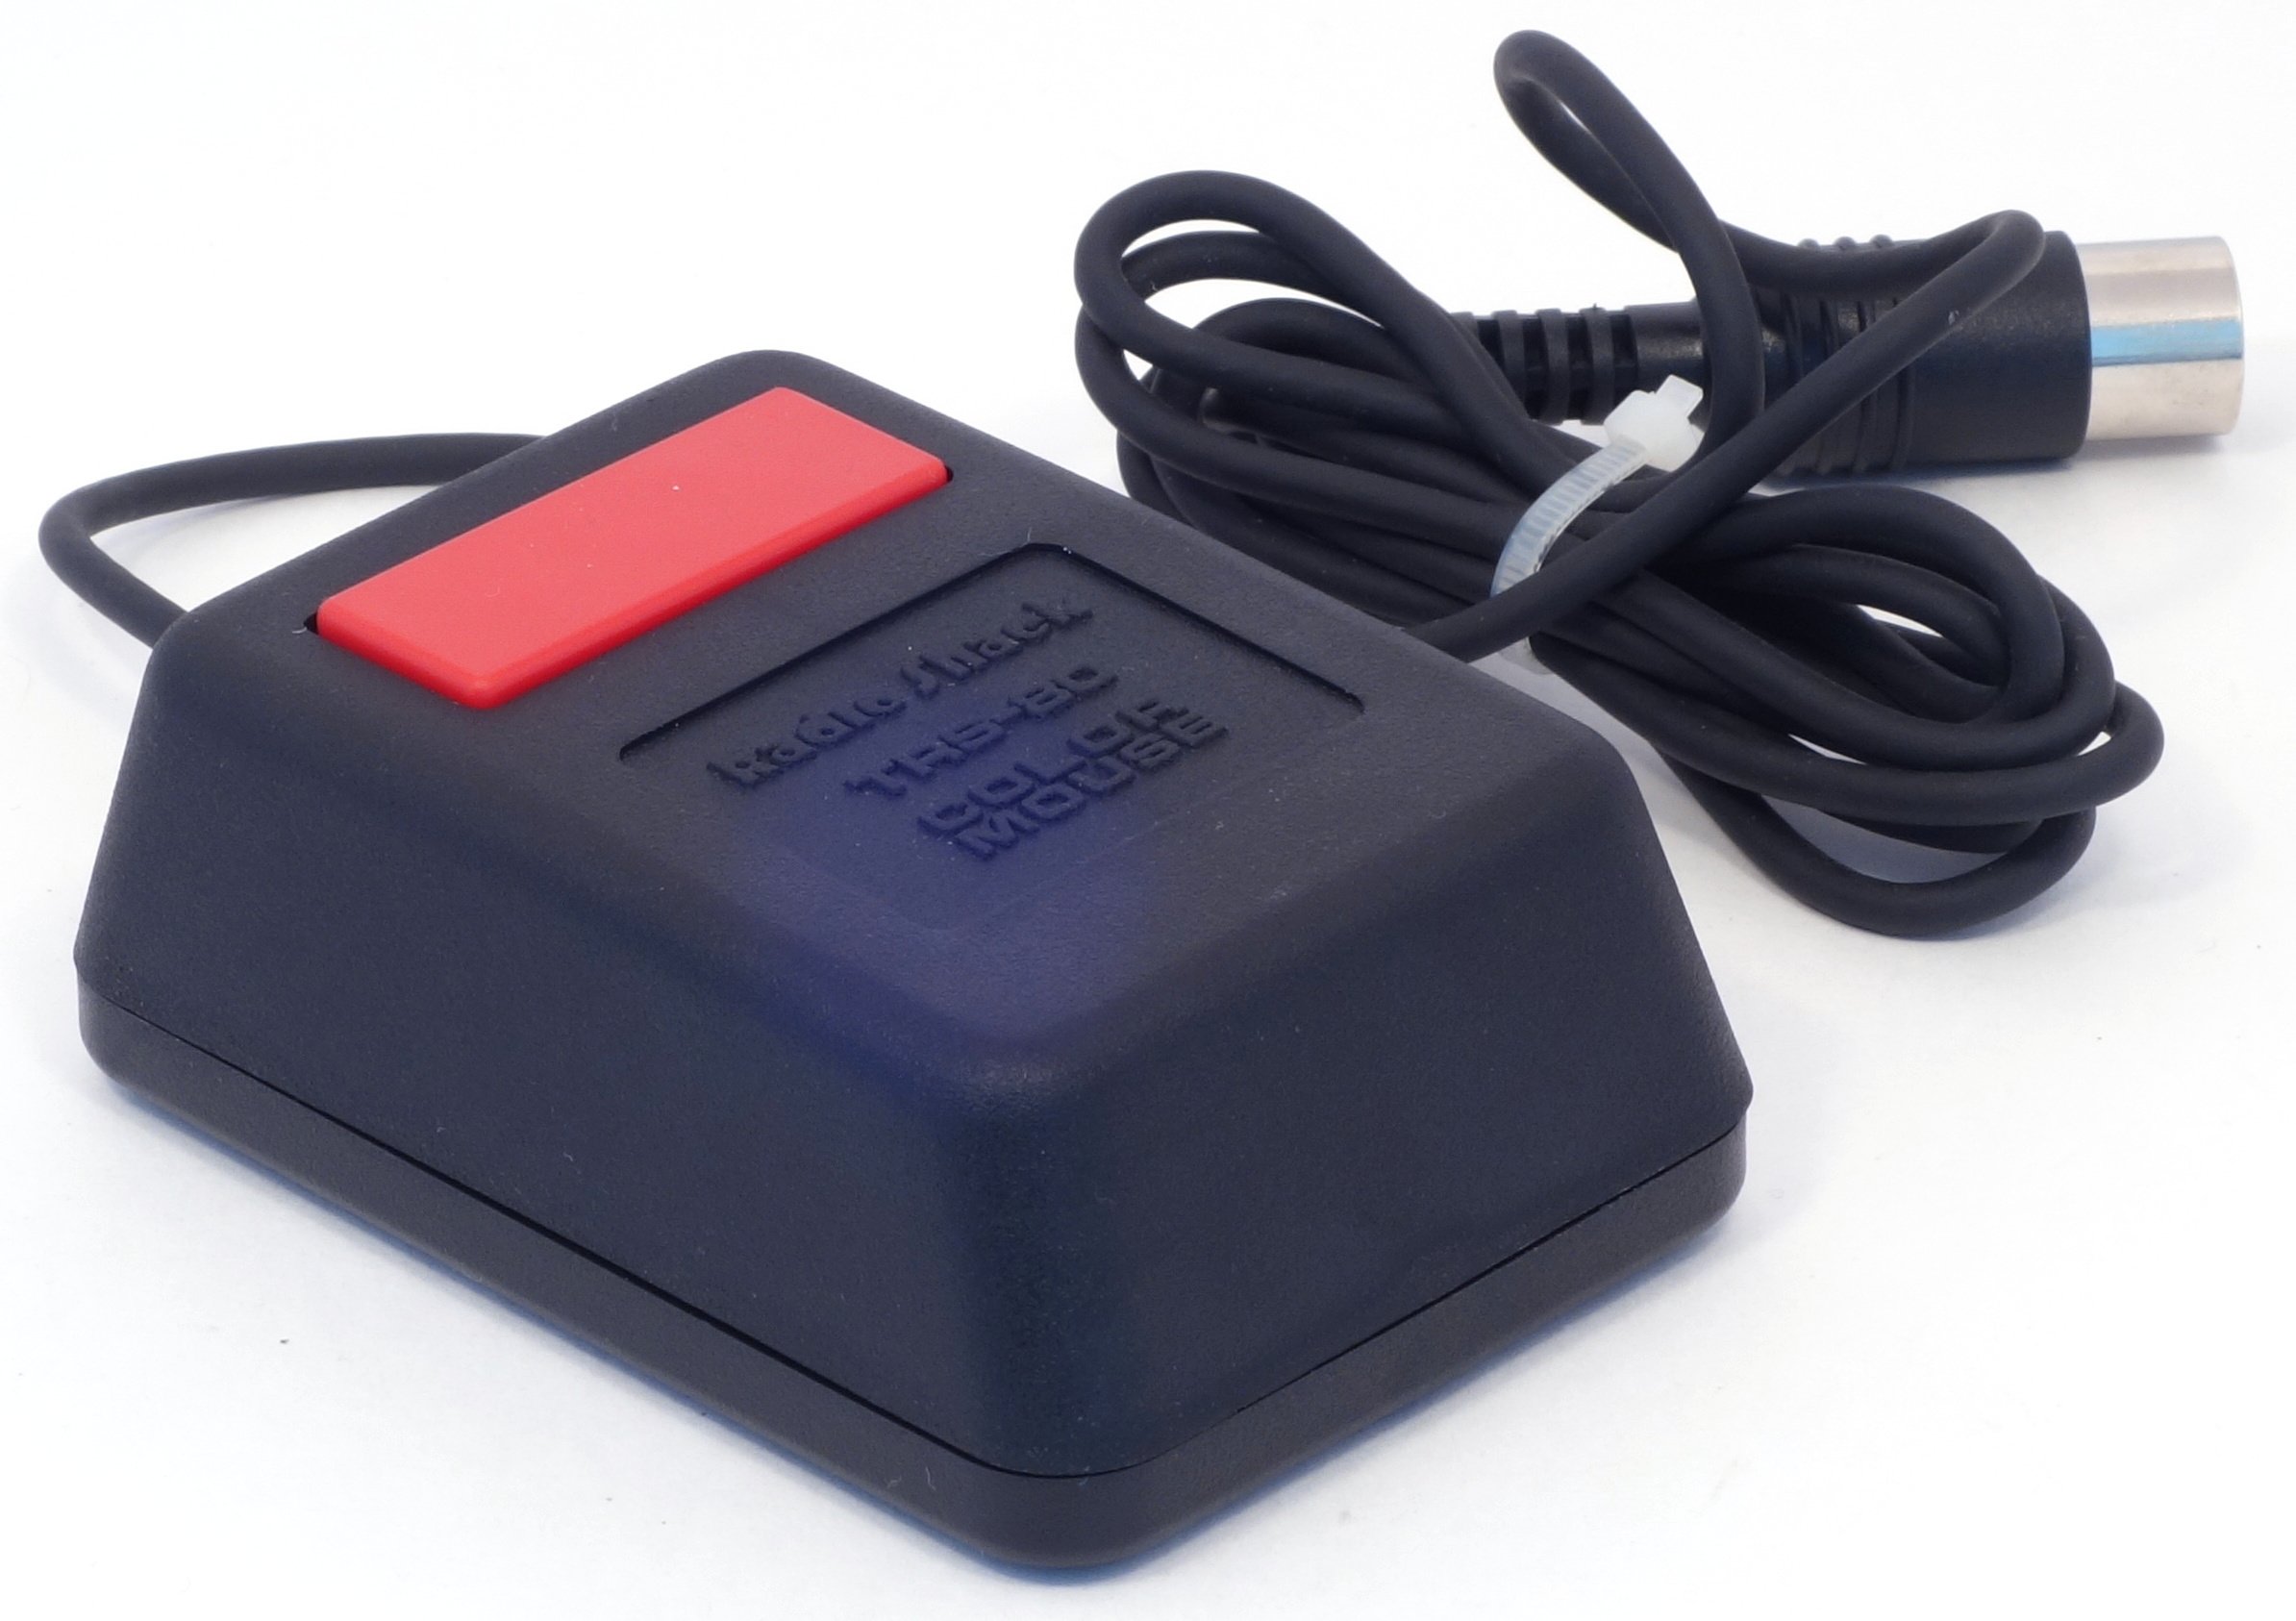
\includegraphics[scale=0.66]{1984_tandy_trs80_color_mouse/pic_30.jpg}
    \caption{Tandy Color Mouse}
    \label{fig:TandyColorMousePic}
\end{figure}

\begin{figure}[h]
    \centering
    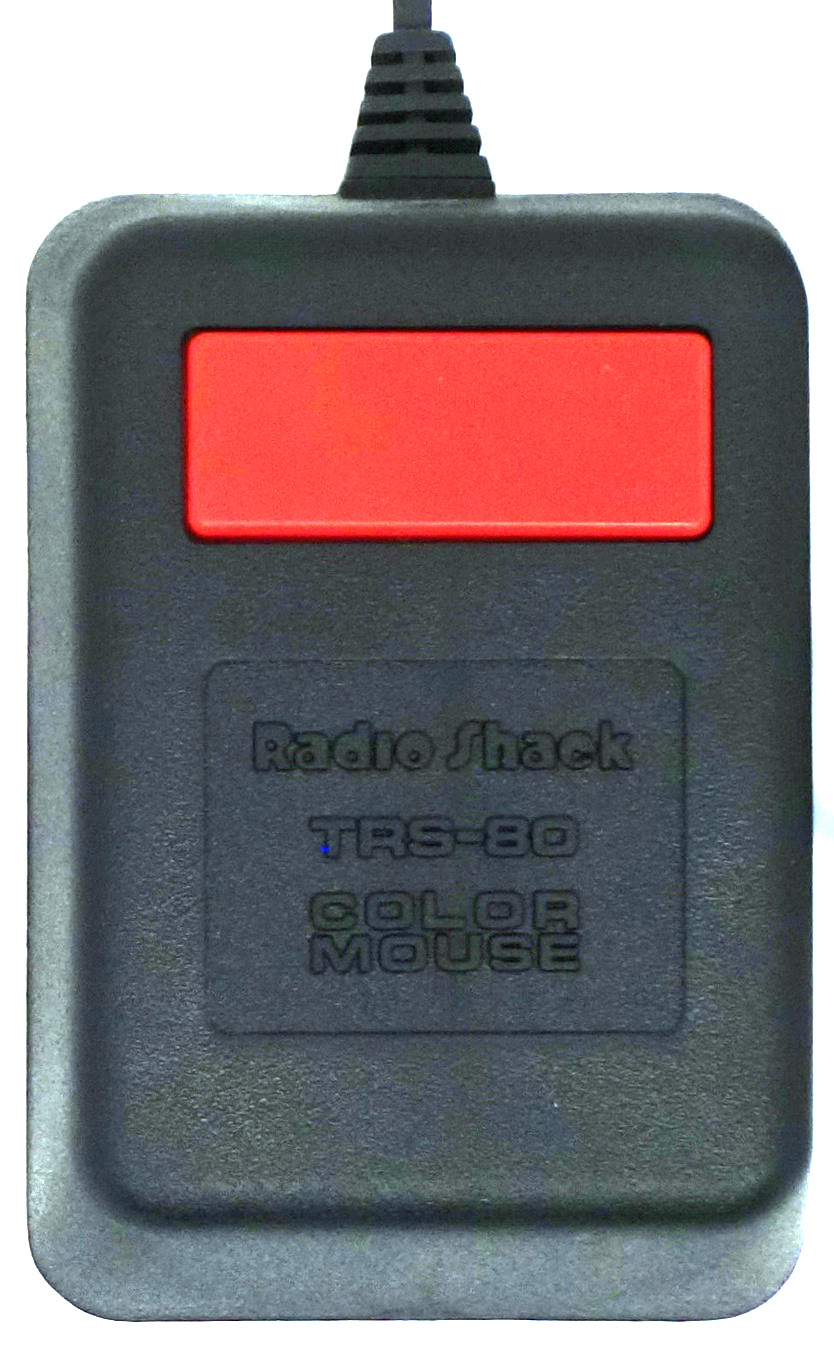
\includegraphics[scale=0.55]{1984_tandy_trs80_color_mouse/top_60.jpg}
    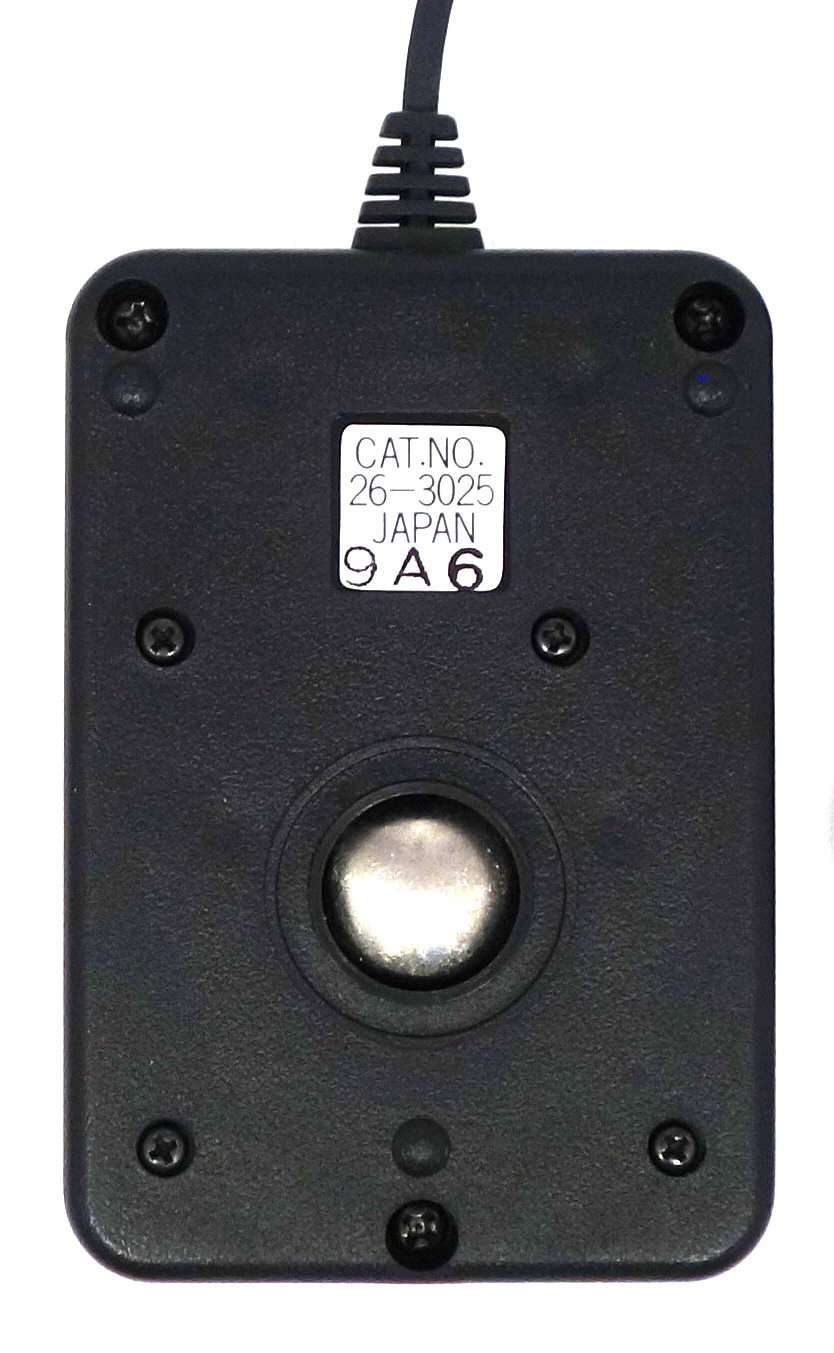
\includegraphics[scale=0.55]{1984_tandy_trs80_color_mouse/bottom_60.jpg}
    \caption{Tandy Color Mouse, top and bottom views}
    \label{fig:TandyColorMouseTopAndBottom}
\end{figure}

The mouse has a single button (fig. \ref{fig:TandyColorMouseTopAndBottom}) similar in shape to that of the Apple Lisa mouse released a year earlier, and the body very closely reproduces the shape of another 1983 mouse -- Sharp MZ-1X10, also manufactured by Alps. The black and red color scheme of the Color Mouse follows the base model of the Tandy Color Computer joystick \cite{hierophant}.

The bottom side shows exactly the same steel ball as the MZ-1X10 has. However, the design of the Color Mouse is much cheaper compared to it: there are no metal balls used as the mouse feet for easier sliding, and no removable ring which would allow removing the ball for cleaning. The only improvement is a plastic insert that protects the wire from damage in place where it exits the mouse body.

The mouse has a small size typical of the 80s (fig. \ref{fig:TandyColorMouseSize}).

\begin{figure}[h]
    \centering
    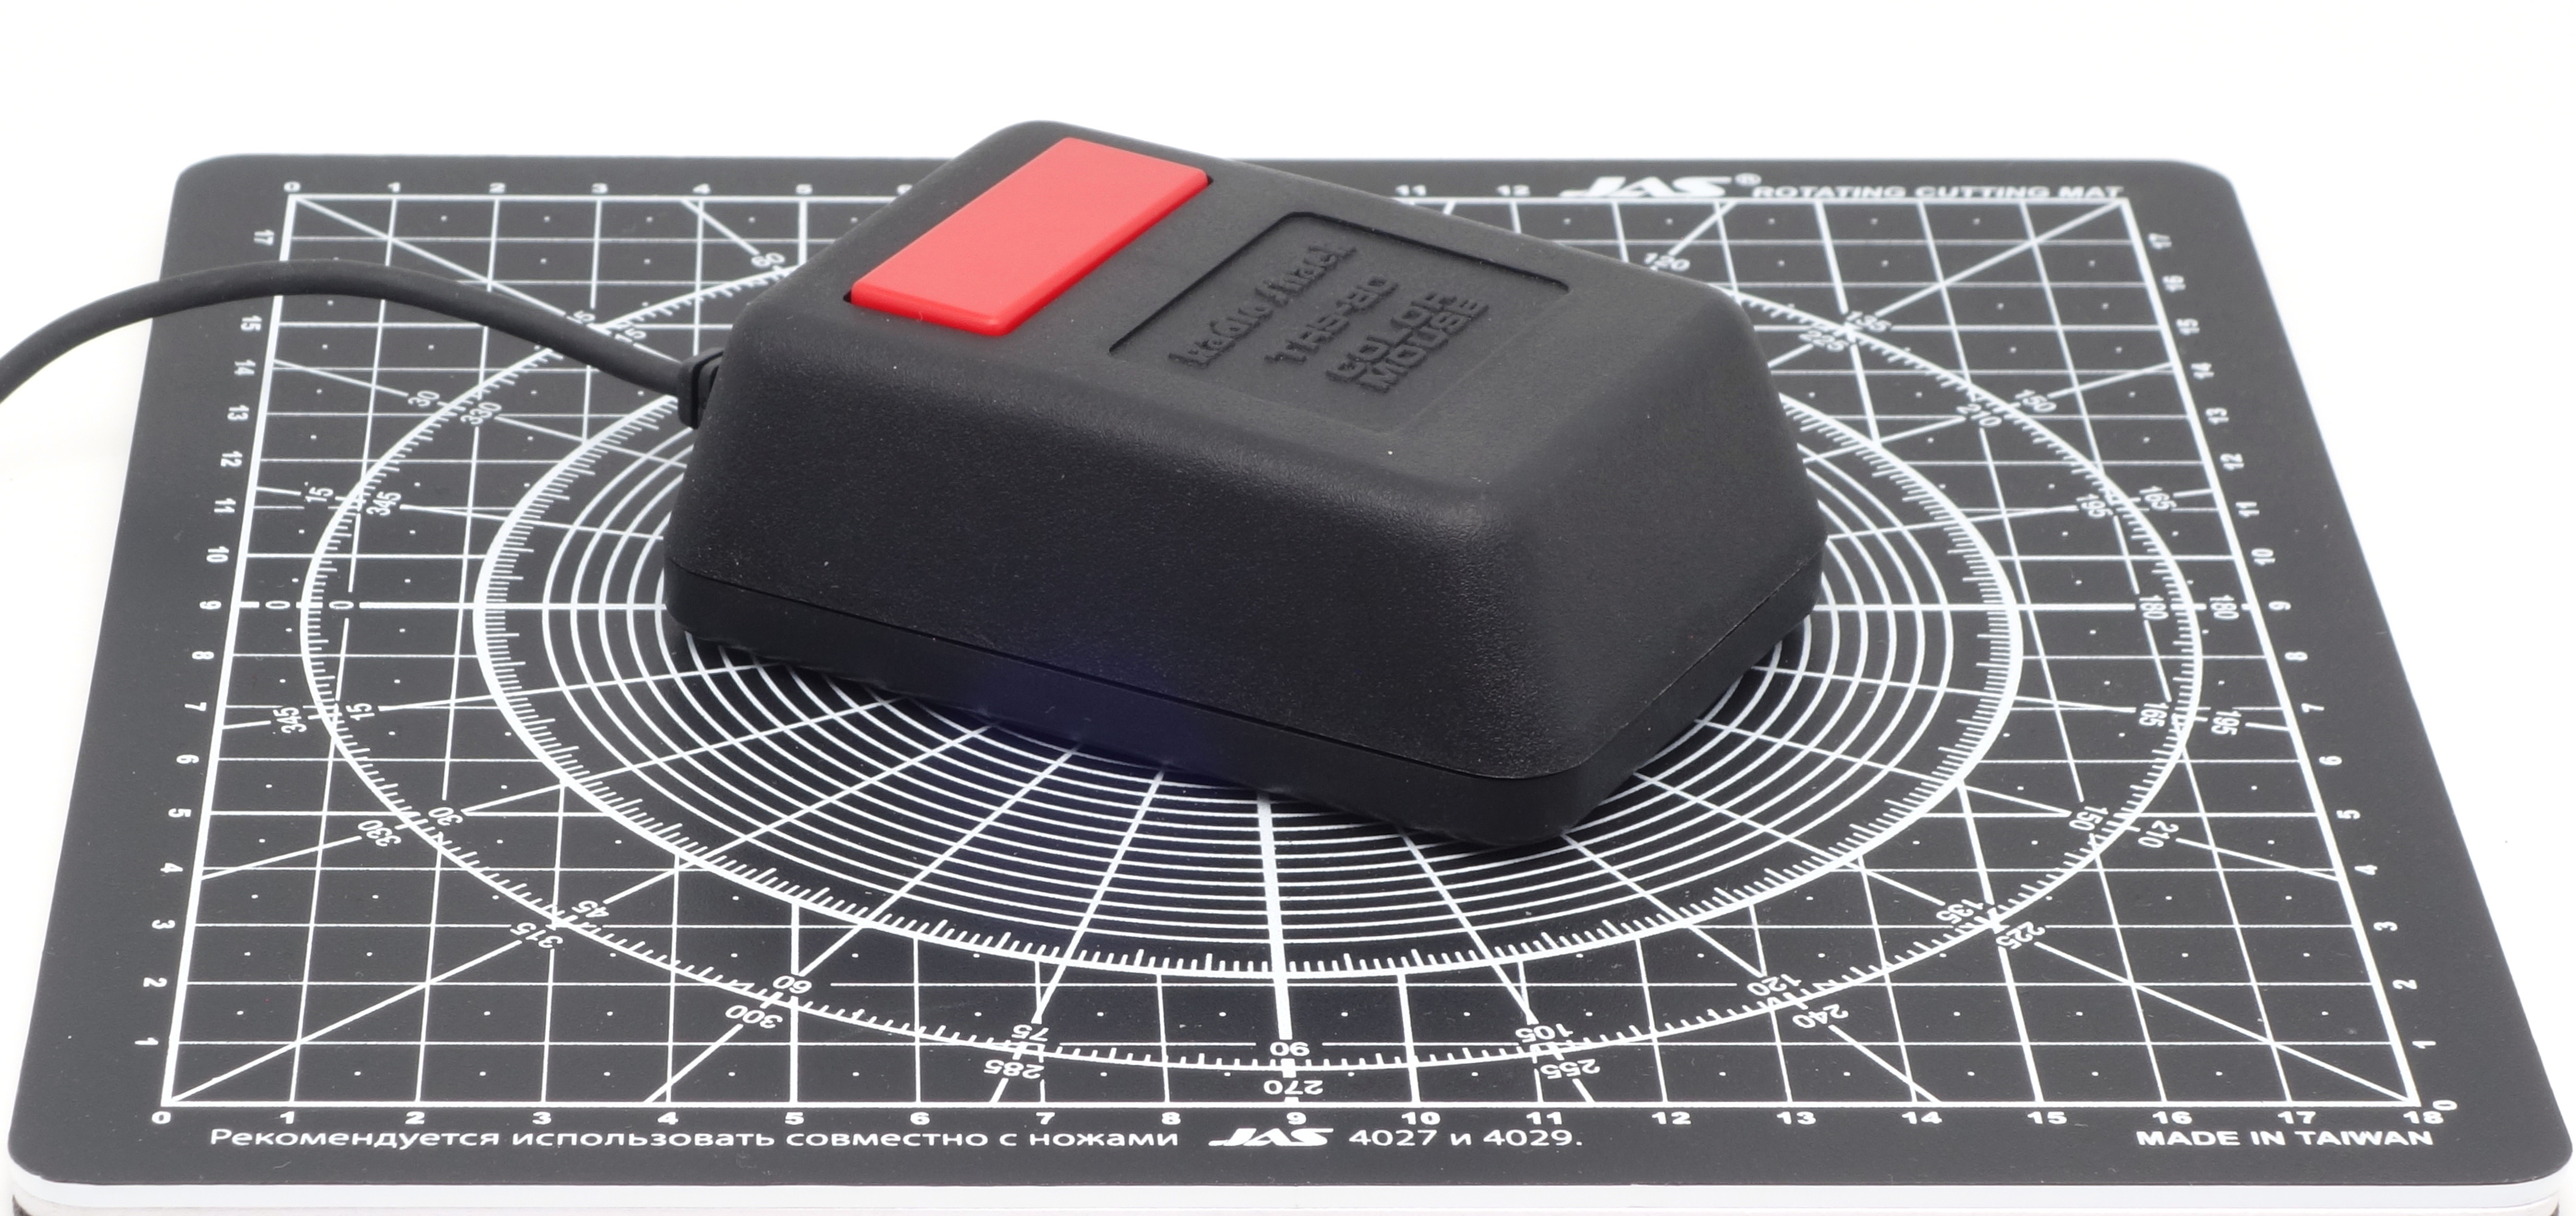
\includegraphics[scale=0.49]{1984_tandy_trs80_color_mouse/size_30.jpg}
    \caption{Tandy Color Mouse on a graduated pad with a grid step of 1~cm}
    \label{fig:TandyColorMouseSize}
\end{figure}

Color Mouse has a fairly simple design; its shape resembles power supply of a player or some other home gadget. Obviously, the beveled back edge should provide a more comfortable palm position, but taking into account the size this does not bring significant improvements to ergonomics (fig. \ref{fig:TandyColorMouseHand}).

As mentioned, the mouse connects to the analog joystick port. As in the case of a joystick, information about each of the two coordinates is encoded in analog form, by the value of the electrical voltage on the corresponding connector pin. It is stated in the user manual, that mouse resolution is 64 <<steps>> along each of two coordinate axes \cite{manual}. Such low resolution is caused by the limitations of the Tandy Color Computer analog-to-digital converter: drivers that allow using real analog joysticks to control mouse cursor were also showing poor positioning accuracy \cite{hierophant}.

\begin{figure}[h]
    \centering
    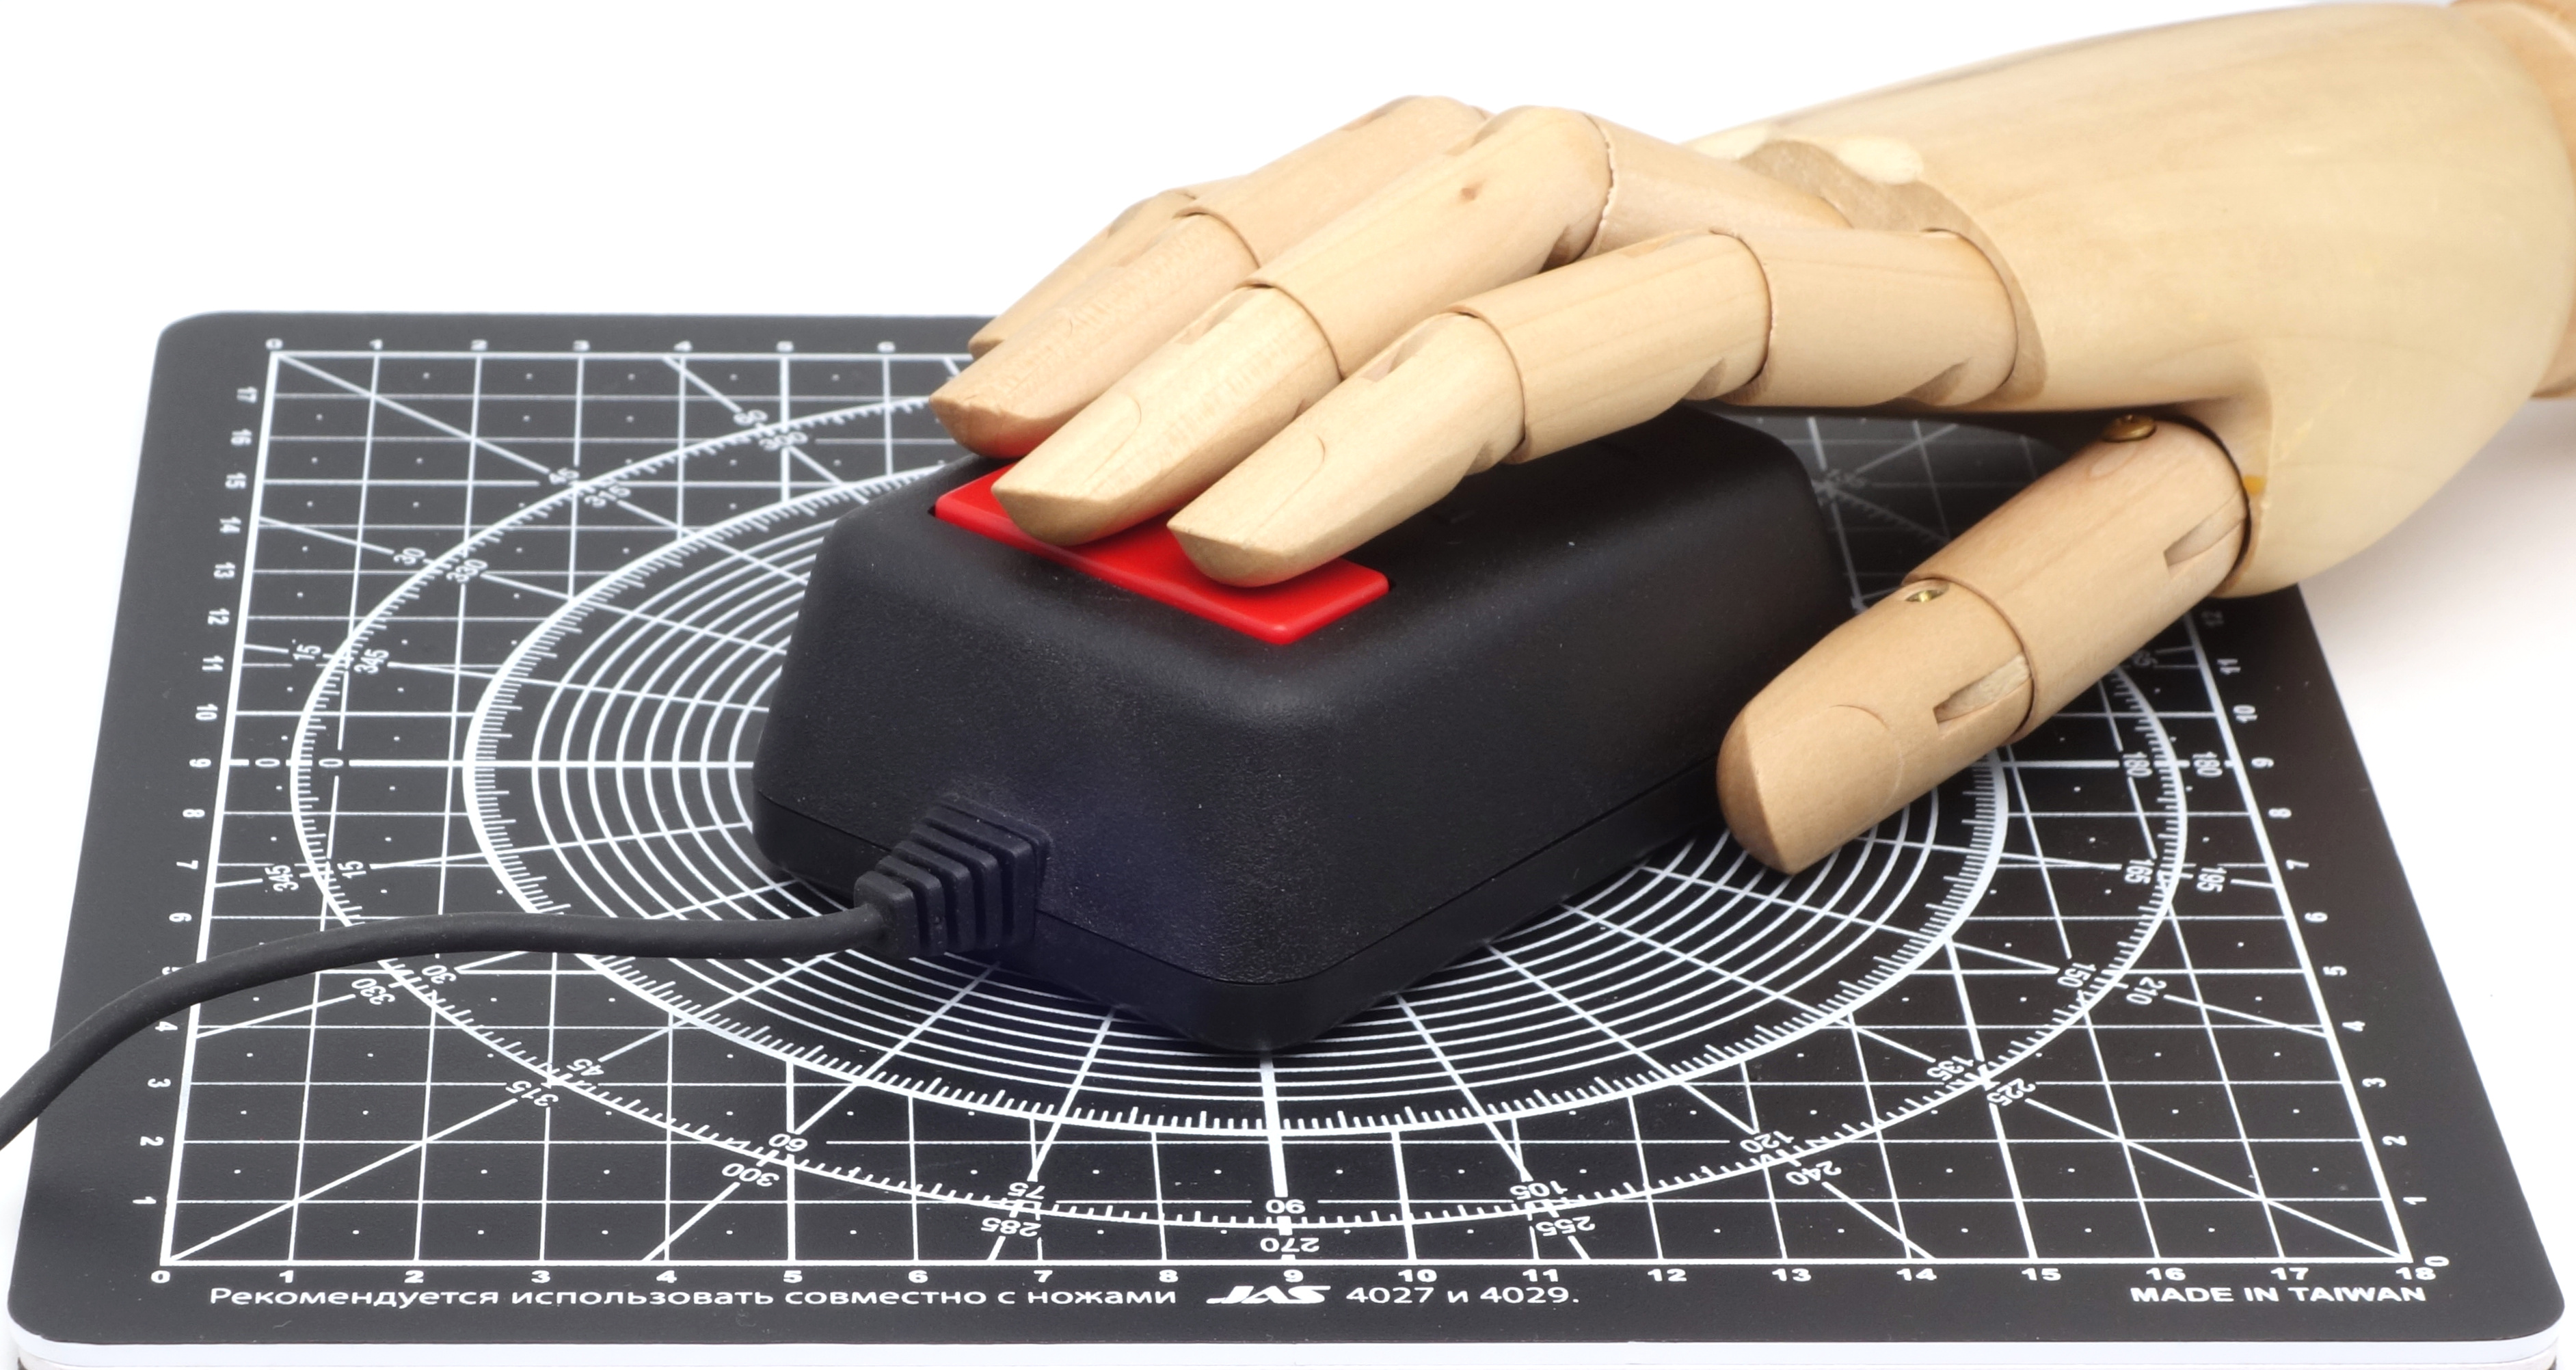
\includegraphics[scale=0.55]{1984_tandy_trs80_color_mouse/hand_30.jpg}
    \caption{Tandy Color Mouse with a human hand model}
    \label{fig:TandyColorMouseHand}
\end{figure}



\begin{figure}[h]
    \centering
    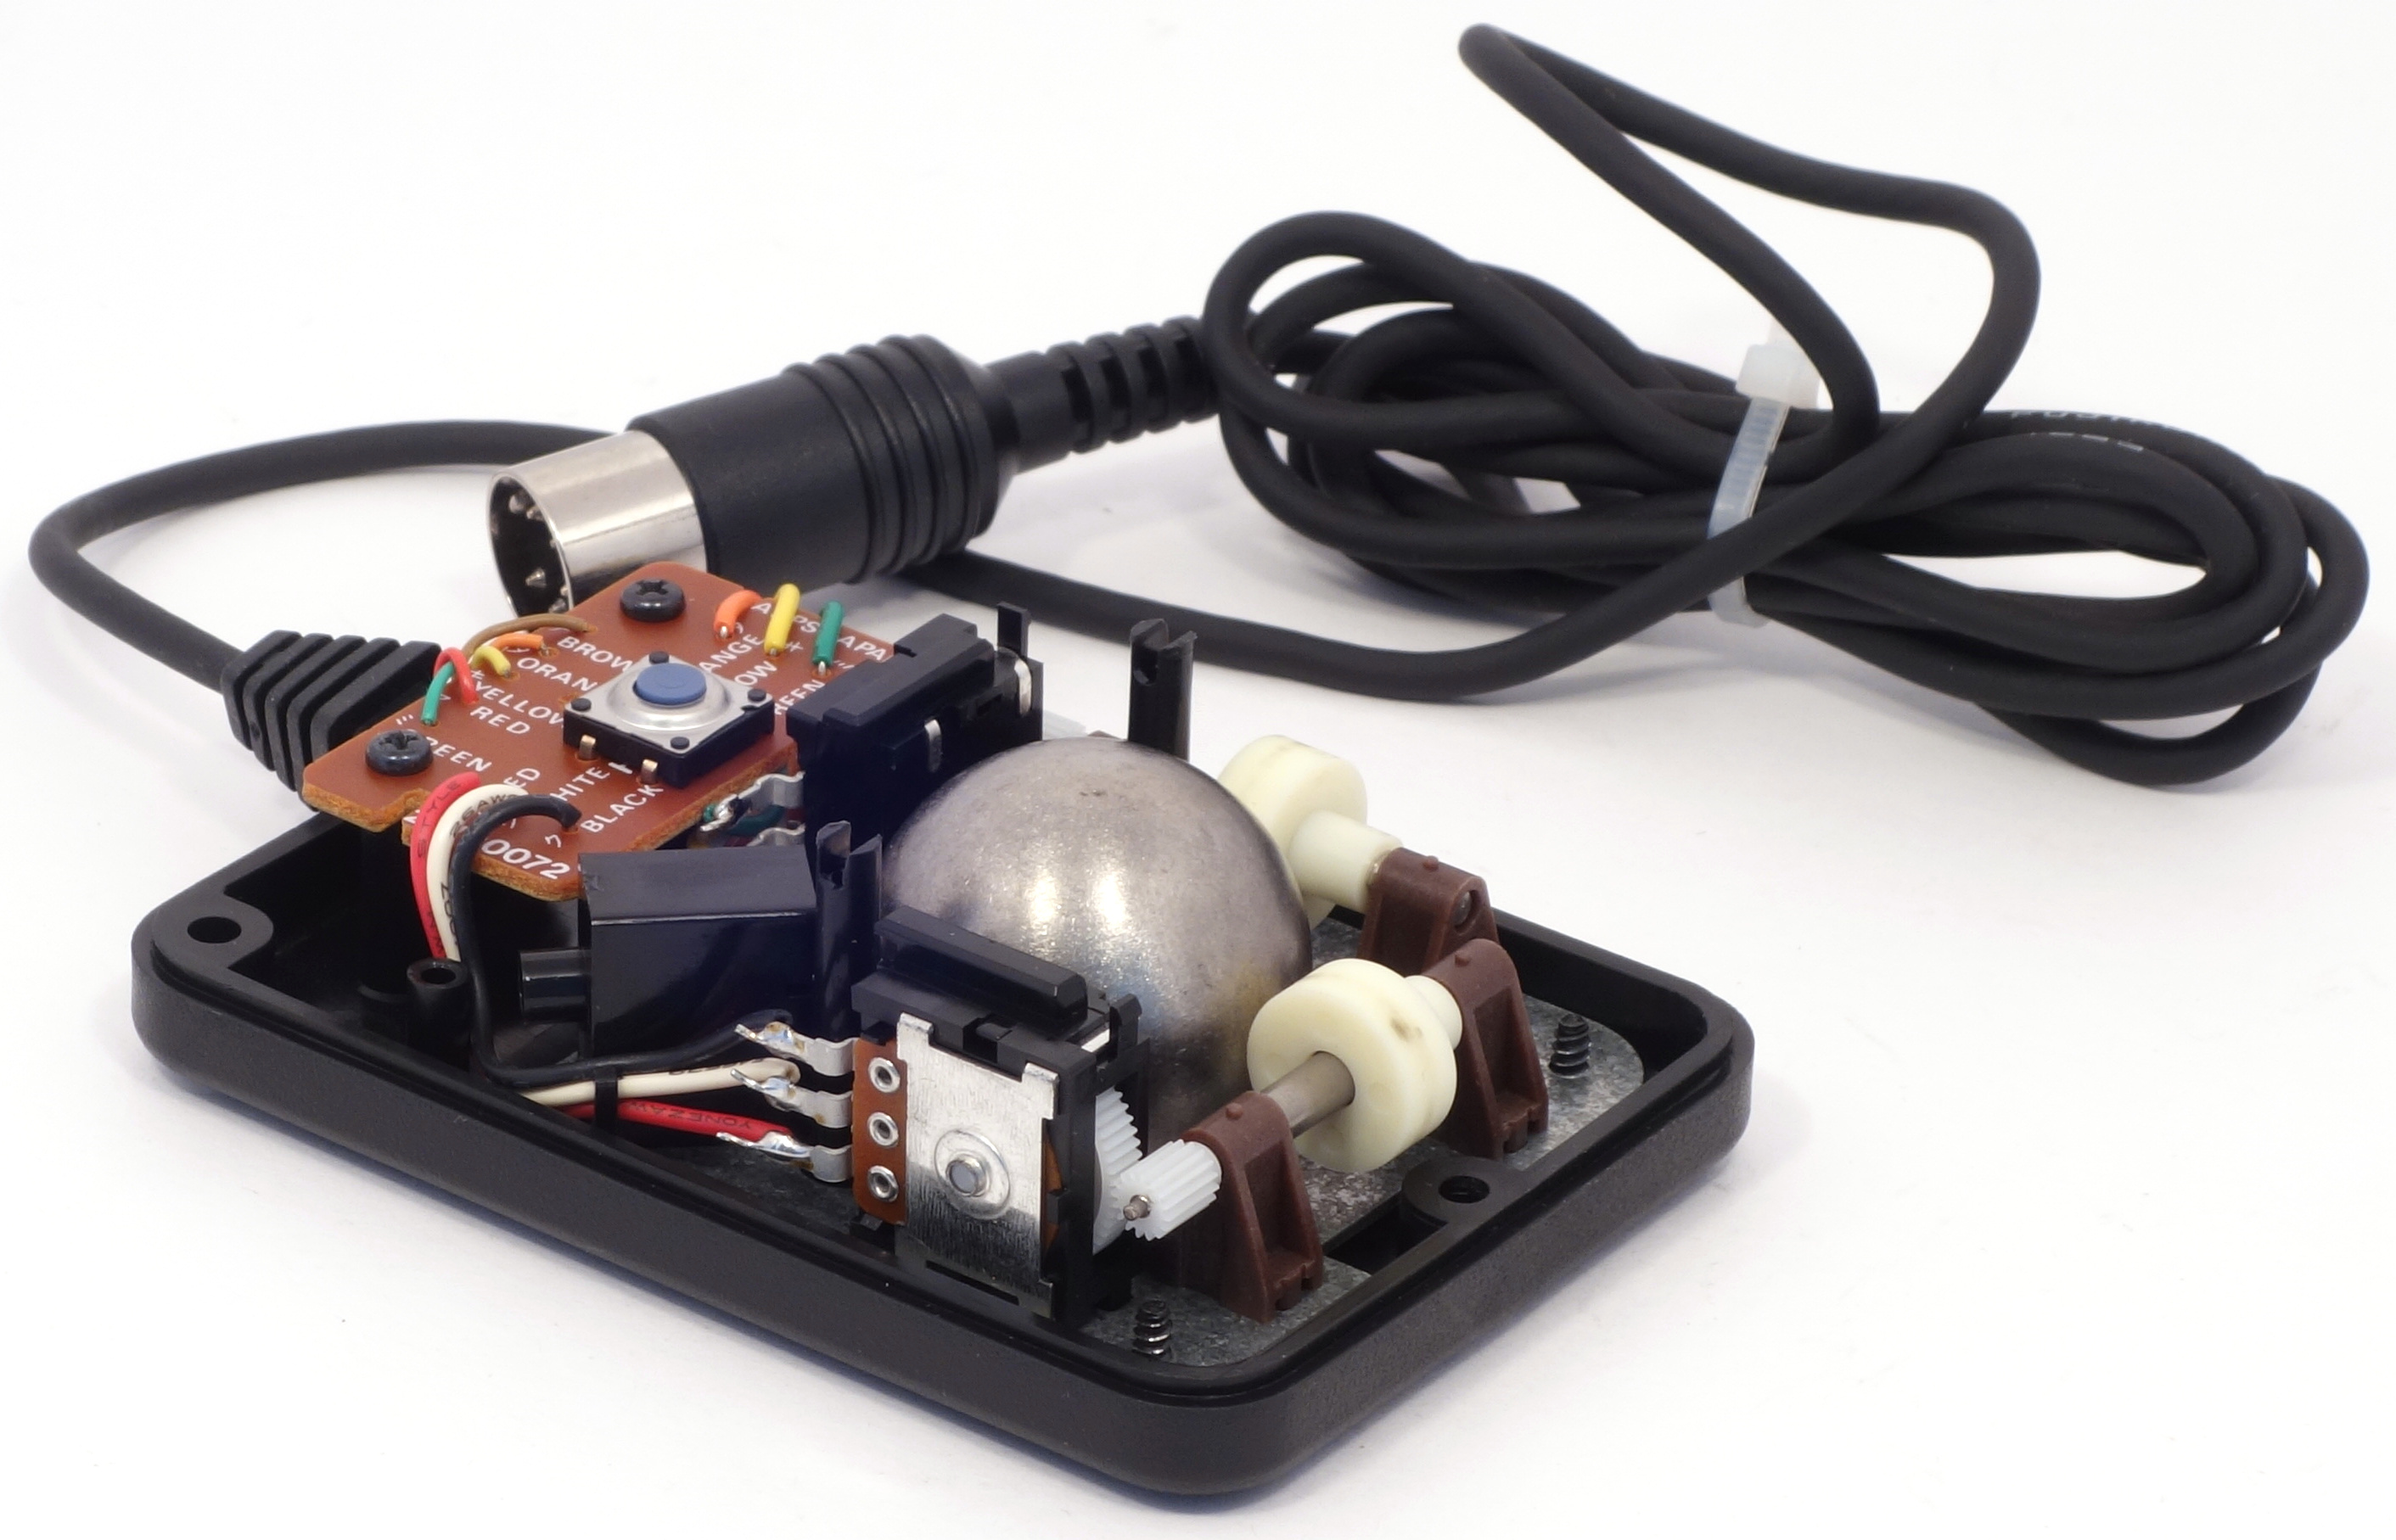
\includegraphics[scale=0.8]{1984_tandy_trs80_color_mouse/inside_30.jpg}
    \caption{Tandy Color Mouse disassembled}
    \label{fig:TandyColorMouseInside}
\end{figure}

Disassembled mouse is shown in fig. \ref{fig:TandyColorMouseInside}. Tandy Color Mouse does not use contact or optomechanical encoders: instead, the ball transmits motion to a pair of potentiometers, just like an analog joystick stick does. Of course, this solution has significant drawbacks: the mouse does not allow calibration, and unlike the joystick, the mouse can't show user that its potentiometers have been moved to the middle position, which should correspond to the location in the center of the mousepad, or that they have reached the edje position. However, since Tandy Color Mouse is an absolute coordinate pointing device, user can see location of the cursor on the screen and place the mouse on more or less appropriate part of the mousepad.

\begin{thebibliography}{9}
\bibitem {manual} TRS-80 COLOR MOUSE For Color Computer Operational Manual \url{https://colorcomputerarchive.com/repo/Documents/Manuals/Hardware/TRS-80%20Color%20Mouse%20%28Tandy%29.pdf}
\bibitem {adv} 1984 Radio Shack Catalog. p. 178 \url{https://www.radioshackcatalogs.com/flipbook/1984_radioshack_catalog.html}, \url{https://web.archive.org/web/20230430161918/https://www.radioshackcatalogs.com/flipbook/catalogs/main/1984/178.jpg}
\bibitem {hierophant} Tandy Color Computer Mice - A Viable Alternative for Tandy 1000s without a Serial Port? January 21, 2016. -- \url{http://nerdlypleasures.blogspot.com/2016/01/tandy-color-computer-mice-viable.html}
\bibitem {wiki} TRS-80 Color Computer -- Wikipedia \url{https://en.wikipedia.org/wiki/TRS-80_Color_Computer}
\end{thebibliography}
\end{document}
